\section {实现内容}
\subsection {光线追踪}
这一部分在第二次小作业中已经基本实现,在本次实验中,对之前的光线追踪渲染器进行进一步修改及扩展。

\subsubsection {多线程下随机数生成}
在之前的作业中使用了C的srand方法种下种子,并调用rand方法来获取伪随机数。在多线程加速的情况下,会导致多个线程产生相同随机数的情况,但这并不是我们想要的结果。

在本次实验中,实现了RNGenerator类,以支持对多线程随机数的生成。RNGenerator 类封装了C++11的随机数生成引擎,并且使用梅森旋转算法\footnote{\url{https://en.wikipedia.org/wiki/Mersenne_Twister}} 来进行随机数的生成。当然,最主要的目标还是要保证不同线程的种子不同。在对RNGenerator 类进行实例化时,将会使用当时的时间及当前线程ID做异或操作,用上述结果作为随机数种子,从而保证了多线程随机数生成的随机性。

\subsubsection {额外渲染对象的支持}
实现了对四边形的支持,使用了[\cite{lagae2005efficient}]所述的光线与四边形快速求交的算法。以此为基础,即可实现对康奈尔盒模型的渲染。

\subsubsection {场景文件}
在本次实验中将场景文件修改为较容易理解且读取的xml文件,在原工程中使用rapidxml库进行xml文件的读入。

\subsection {蒙特卡洛路径追踪}
路径追踪\footnote{\url{https://en.wikipedia.org/wiki/Path_tracing}}是一种对真实世界下全局光照的蒙特卡洛渲染方法,笼统来讲,该算法利用蒙特卡洛方法对渲染方程进行近似,从而达到对真实情况的逼近。在本次实验中,路径追踪渲染器用来作为直接/非直接光照的数据生成器及用来对比的Ground-Truth 数据生成器。

\subsubsection {渲染方程}
渲染方程\footnote{\url{https://en.wikipedia.org/wiki/Rendering_equation}} 于1986年被引入计算机图形学,在不考虑波长$\lambda$及时间$t$的情况下,其形式如下:
\[
    L_{o}(\bm{x}, \omega_{o})=L_{e}(\bm{x}, \omega_{0})+\int_{\Omega}f_{r}(\bm{x}, \omega_{i}, \omega_{o})L_{i}(\bm{x}, \omega_{i})(\omega_{i}\cdot\bm{n})d\omega_{i}
\]
其中
\begin{itemize}[noitemsep]
    \item $L_{o}(\bm{x}, \omega_{o})$ 代表在位置$\bm{x}$以及角度$\omega_{o}$的出射光
    \item $L_{e}(\bm{x}, \omega_{o})$ 代表上述位置及方向发出的光
    \item $\int_{\Omega} ...d\omega_{i}$ 代表入射方向半球的无穷小累加和
    \item $f_{r}(\bm{x}, \omega_{i}, \omega_{o})$ 是BRDF,也即在该点从入射方向到出射方向光的反射比例
    \item $L_{i}(\bm{x}, \omega_{i})$ 代表该点的入射光位置及方向$\omega_{i}$
\end{itemize}

\subsubsection {重要性采样}
在蒙特卡洛方法模拟积分时,采用重要性采样方法会使蒙特卡洛方法得到结果的方差减小,从而使算法更好更快地收敛至正确结果。

在路径追踪的过程中,当追踪光线与某物体存在一个交点时,需要随机确定一个反射方向从而继续追踪,此时就需要使用重要性采样来对不同的BRDF进行方向的选择。方向向量$\omega$可以由天顶角$\theta$及方位角$\phi$ 确定,接下来介绍两种BRDF 的重要性采样方法\footnote{参考自\url{https://www.cs.virginia.edu/~jdl/importance.doc}}。

如果该物体的BRDF是Lambertian,也即$f_{r}(\bm{x}, \omega_{i}, \omega_{o})=\frac{\rho}{\pi}$。假设$u,v$是两个属于$[0,1]$且均匀分布的随机数,那么
\[
    (\theta, \phi)=(arccos(\sqrt{1-u}), 2\pi v)
\]
概率分布函数为
\[
    pdf(\omega_{i})=\frac{cos(\theta)}{\pi}
\]

如果该物体的BRDF是Phong,也即$f_{r}(\bm{x}, \omega_{i}, \omega_{o})=\frac{k_{d}}{\pi}+k_{s}\frac{(n+2)}{2\pi}cos^{n}(\alpha)$。 由于表达式的前半部分与Lambertian一致,我们只讨论后半部分的情况。$u,v$的定义同上,则
\[
    (\theta, \phi)=(arccos(u^{\frac{1}{n+1}}), 2\pi v)
\]
概率分布函数为
\[
    pdf(\omega_{i})=\frac{n+1}{2\pi}cos^{n}(\alpha)
\]
其中$\alpha$为$\omega_{o}$与$\bm{n}$所成的夹角。

\subsubsection {直接光照\& 非直接光照}
由于在之后的实验中,会对场景中每个物体的直接光照及非直接光照进行训练,所以需要将当前的渲染方法拆成直接光照值和非直接光照值。

当追踪光线与某物体存在一个交点时,每次只需递归跟踪一条路径,现在追踪两条:一条指向光源$\omega_{direct}$,另一条与之前相同,仍然通过重要性采样随机进行跟踪$\omega_{indirect}$。其中,$\omega_{direct}$路径无需继续递归,只计算光源的发射光,$\omega_{indirect}$路径则继续递归跟踪下去。计算直接光照的伪代码见算法~\ref{alg:direct}:
\begin{algorithm}
\begin{algorithmic}
    \STATE $\omega_{i},pdf=$luminaireSample($x,\bm{n}$)
    \STATE $y=$traceRay($x,\omega_{i}$)
    \RETURN brdf($x,\omega_{i},\omega_{r}$)$\cdot$emittedRadiance($y,-\omega_{i}$)$/pdf$
\end{algorithmic}
\caption{directRadianceEst($x,\omega_{r}$)}
\label{alg:direct}
\end{algorithm}
这里提到了对光源的采样以及概率密度分布函数问题,这个问题将在下一小节说明。计算非直接光照的伪代码见算法~\ref{alg:indirect}:
\begin{algorithm}[h]
\begin{algorithmic}
    \IF {random()$<$survivalProbability}
        \STATE $\omega_{i},pdf=$brdfSample($x,\bm{n}$)
        \STATE $y=$traceRay($x,\omega_{i}$)
        \RETURN brdf($x,\omega_{i},\omega_{r}$)$\cdot$reflectedRadianceEst($y,-\omega_{i}$)$/(pdf\cdot$survivalProbability$)$
    \ELSE
        \RETURN 0
    \ENDIF
\end{algorithmic}
\caption{indirectRadianceEst($x,\omega_{r}$)}
\label{alg:indirect}
\end{algorithm}

由上述两个算法就可以将直接光照及非直接光照拆开,为之后的训练打好基础。图~\ref{fig:direct_indirect}由我们的渲染器给出,可以看出一张渲染出的全局光照图像是局部光照与辐射度的和。
\begin{figure}[h]
    \centering
    \begin{subfigure}{0.3\textwidth}
        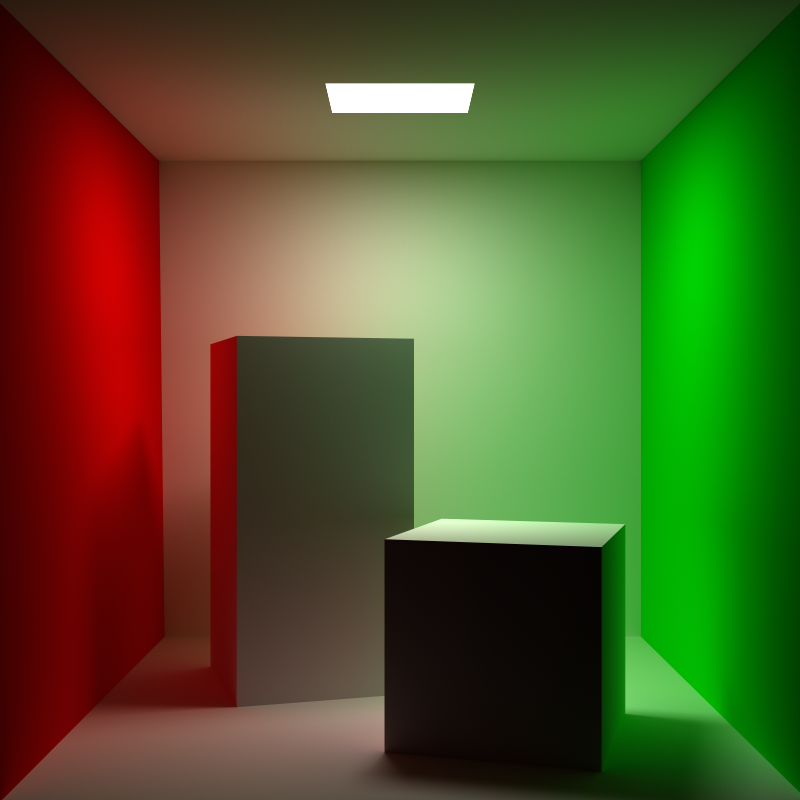
\includegraphics[width=\textwidth]{img/all.png}
        \caption{全局光照}
    \end{subfigure}
    ~
    \begin{subfigure}{0.3\textwidth}
        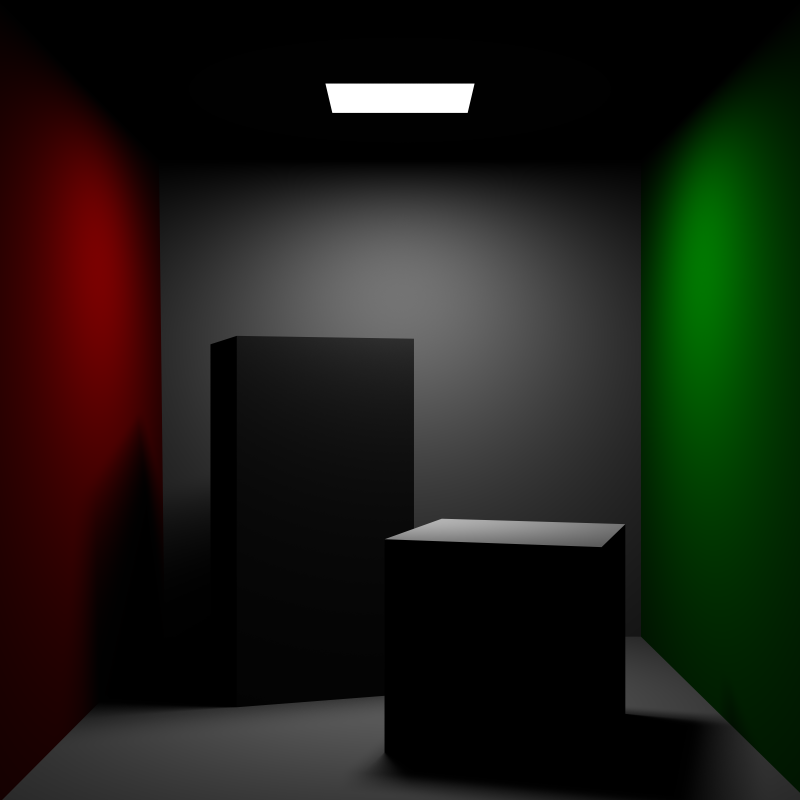
\includegraphics[width=\textwidth]{img/direct.png}
        \caption{直接光照}
    \end{subfigure}
    ~
    \begin{subfigure}{0.3\textwidth}
        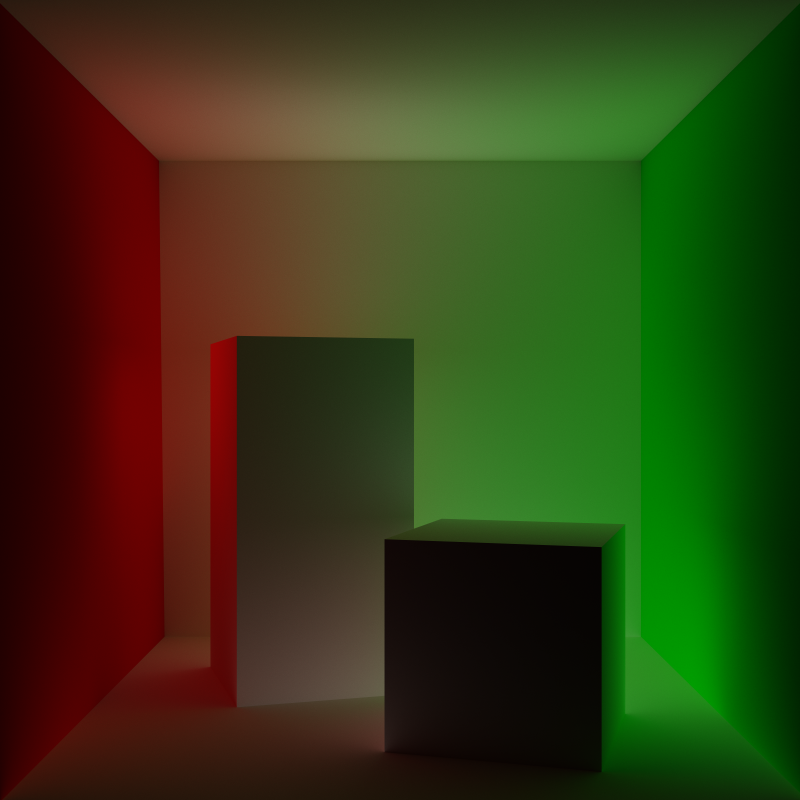
\includegraphics[width=\textwidth]{img/indirect.png}
        \caption{非直接光照}
    \end{subfigure}
    \caption{全局光照=直接光照+非直接光照}
    \label{fig:direct_indirect}
\end{figure}

这样做还有一个好处,由于朴素蒙特卡洛路径追踪法只能在追踪路径与光源由交点时,才能计算出光照值,如果场景中的光源面积很小甚至就是一个点光源,那么这种方法会导致渲染结果偏暗甚至全黑。将直接光照与非直接光照拆开来计算可以避免这个问题,图~\ref{fig:plain_distribution} 可以看出,在spp相同的情况下,这种方法名明显强于朴素方法。
\begin{figure}[h]
    \centering
    \begin{subfigure}{0.4\textwidth}
        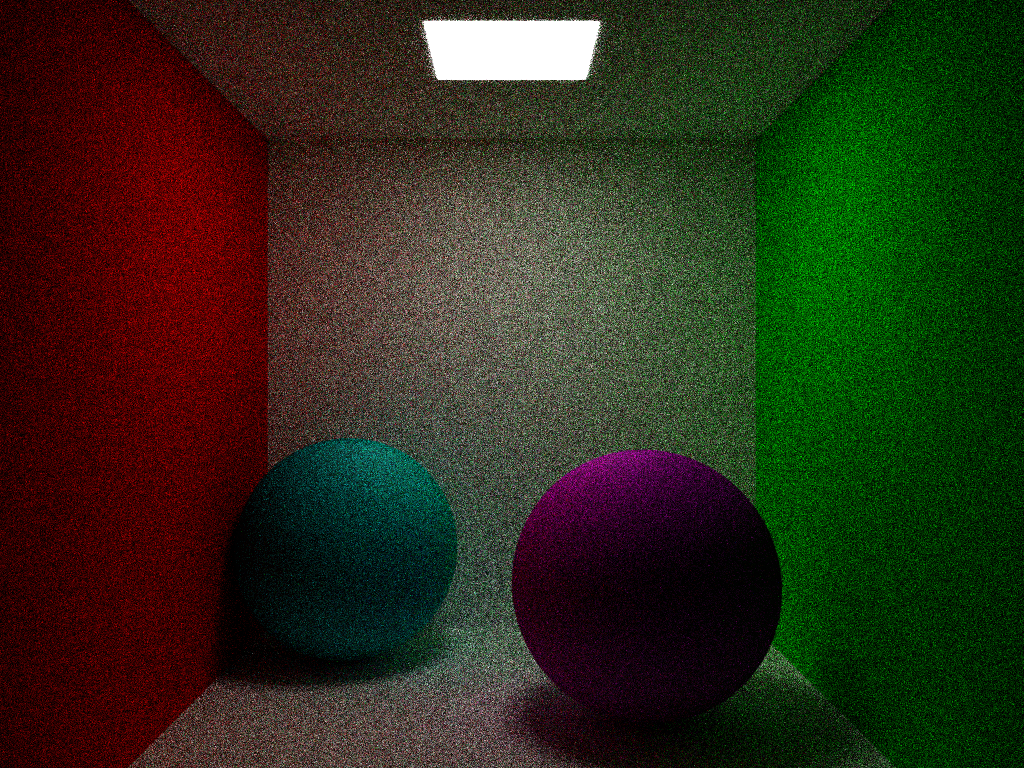
\includegraphics[width=\textwidth]{img/plain_mcpt.png}
        \caption{朴素方法,spp=200}
    \end{subfigure}
    ~
    \begin{subfigure}{0.4\textwidth}
        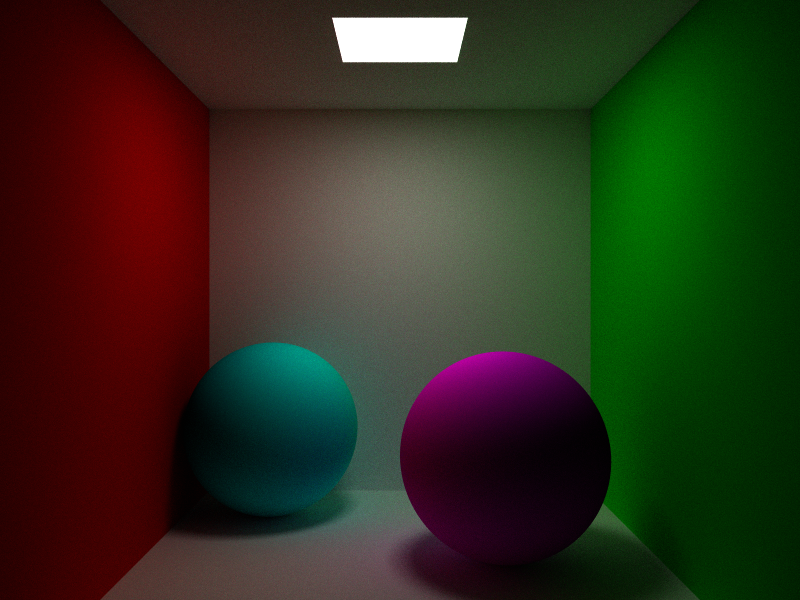
\includegraphics[width=\textwidth]{img/distribution_mcpt.png}
        \caption{分别计算,spp=200}
    \end{subfigure}
    \caption{朴素方法渲染出图像的方差相较于分别计算的明显偏大}
    \label{fig:plain_distribution}
\end{figure}

\subsubsection {直接光照中的光源采样}
由[\cite{shirley1996monte}]所述,直接光照的积分表达式为:
\[
    L_{d}(\bm{x},\hat{\omega})=\int_{\chi}g(\bm{x},\bm{x^{'}})f_{r}(\bm{x},\hat{\omega},\hat{\omega}^{'})L_{e}(\bm{x^{'}},\hat{\omega}^{'})(-\hat{\omega}^{'}\cdot\hat{n})\frac{\hat{\omega}^{'}\cdot\hat{n}^{'}}{||\vv{\bm{x}-\bm{x^{'}}}||^{2}}dA(x^{'})
\]
其中
\begin{itemize}[noitemsep]
    \item $\chi$表示光源表面所有点的集合
    \item $g(\bm{x},\bm{x^{'}})$代表从点$\bm{x}$是否能看到$\bm{x^{'}}$。如果能,则值为$1$;反之为$0$
\end{itemize}
由蒙特卡洛积分的近似表达式(重要性采样):
\[
    \int_{S}f(\psi^{'})d\mu (\psi^{'})\approx\frac{1}{N}\sum_{i=1}^{N}\frac{f(\psi^{'})}{p(\psi^{'})}
\]
可以得到:
\[
    L_{d}(\bm{x},\hat{\omega})\approx \frac{1}{N}\sum_{i=1}^{N}g(\bm{x},\bm{x^{'}})f_{r}(\bm{x},\hat{\omega},\hat{\omega}^{'})L_{e}(\bm{x^{'}},\hat{\omega}^{'})(-\hat{\omega}^{'}\cdot\hat{n})\frac{\hat{\omega}^{'}\cdot\hat{n}^{'}}{p(\bm{x^{'}})||\vv{\bm{x}-\bm{x^{'}}}||^{2}}
\]
其中$\bm{x}^{'}\sim p$

所以问题就又简化为重要性采样及求概率分布函数的问题了。在本次实验中实现了矩形面光源,采样方法即为在矩形中随机采一个点,表示为
\[
    \bm{x^{'}}=\bm{x_{0}}+\xi_{1}\vv{v_{1}}+\xi_{2}\vv{v_{2}}
\]
其中,$\bm{x_{0}}$为矩形的一角,$\bm{v_{1}},\bm{v_{2}}$为边向量。

在本次实验中参考了[\cite{shirley1996monte}]的方法,将概率分布函数设置为:
\[
    p(\bm{x^{'}})=\frac{2}{||\vv{v_{1}}\times\vv{v_{2}}||}
\]
就完成了对光源的采样。

\subsection {数据生成}
我们使用上一节介绍的蒙特卡洛路径追踪渲染器作为数据生成的来源。
\subsubsection {数据结构}
每条数据都由一个$12+n$维的输入向量及一个$3$维的颜色值组成,其中输入向量包括:
\begin{itemize}[noitemsep]
    \item 追踪路径与物体的交点
    \item 观察方向
    \item 光源位置
    \item 交点法向
    \item brdf参数(维度视情况而定)
\end{itemize}
用来训练的数据根据不同物体分成不同的类别,以便之后训练。

\subsubsection {数据完整性}
由于计算能力有限,无法做到像[\cite{ren2013global}]中利用200个PC结点组成的集群进行数据生成及训练,所以考虑在保证数据完整性的情况下尽可能少地生成数据。首先,我尝试在场景中任取$N_{v}=200$个视点,每个视点随机在球面上选取$N_{dir}=6000$个方向进行数据生成。这样做会导致场景中的某些角落并没有收集到太多的数据,从而违反了数据的完整性。为了使场景中更多的位置都能被覆盖到,可以考虑将二维中的抖动采样应用到三维中:将场景分为$N_{v}=N_{dx}\times N_{dy}\times N_{dz}=15\times 15\times 15$ 个小块,在每块中随机选取一个视点,再随机选取$N_{dir}=1200$个方向进行数据生成。在选取视点的过程中舍弃掉一些在封闭物体内部,没有贡献的点。这样一来,就可以使生成的数据更加完整,从而使得训练效果更准确。 在本次实验中,共有约$7,000,000$条数据参与训练。

\subsection {训练}
\subsubsection {原理介绍}
由[\cite{ren2013global}]所述,固定场景的辐射度函数由如下三个基本属性作为自变量构成:路径与物体的交点、观察方向、光源位置。但如果只用这三个自变量来表达辐射度函数,又会使函数的表达变得非常复杂,所以考虑额外引入两个自变量:交点法向和brdf 参数,虽然它们可以由基本属性隐式地表达出来,但由于会使函数变得比较复杂,而且这两个变量也很容易计算,所以就将它们与基本属性放在一起,构成一组增强属性,从而降低了辐射度函数表达起来的难度。也正是由于辐射度函数可以由之前所述的增强属性表示,故可以通过非线性回归方法进行训练及预测。

同样地,直接光照函数的自变量与上述增强属性相同,所以也可以用同样的办法进行操作。并且这种做法也冲破了原论文中光源形态只能为点光源的限制,可以支持一些面光源。

\subsubsection {训练细节}
在本次实验中使用Matlab的神经网络工具包对全连接网络进行训练,网络结构如图~\ref{fig:neural_network},由四层组成:输入层为上一节介绍的输入向量;隐藏层由两个分别包含20个、10个结点的层组成;输出层为三维的颜色值。
\begin{figure}[h]
    \centering
    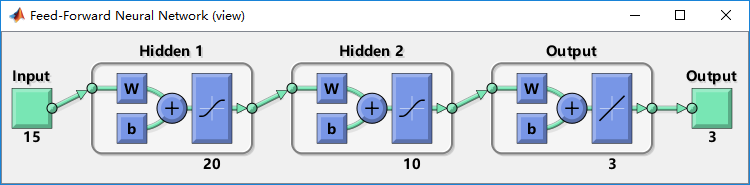
\includegraphics[width=0.8\textwidth]{img/nn.png}
    \caption{全连接网络结构}
    \label{fig:neural_network}
\end{figure}

训练方法采用Levenberg-Marquardt算法\footnote{\url{https://en.wikipedia.org/wiki/Levenberg-Marquardt_algorithm}},最大迭代次数为$1000$。

\subsection {实时渲染}
实时的渲染算法在OpenGL中实现,其中网络权重信息作为纹理信息输入至显存,在shader中对神经网络进行预测,计算出颜色值并显示。

图~\ref{fig:prediction_groundtruth}显示了预测结果与真实渲染结果的对比图。
\begin{figure}[h]
    \centering
    \begin{subfigure}{0.4\textwidth}
        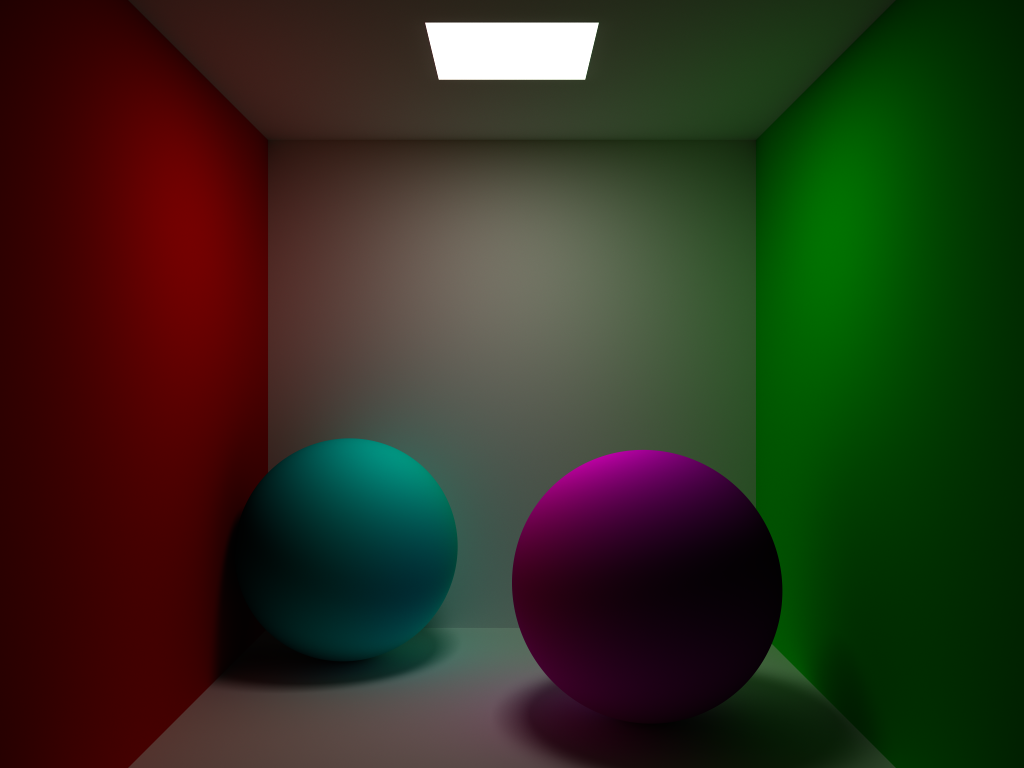
\includegraphics[width=\textwidth]{img/ground_truth.png}
        \caption{Ground truth}
    \end{subfigure}
    ~
    \begin{subfigure}{0.4\textwidth}
        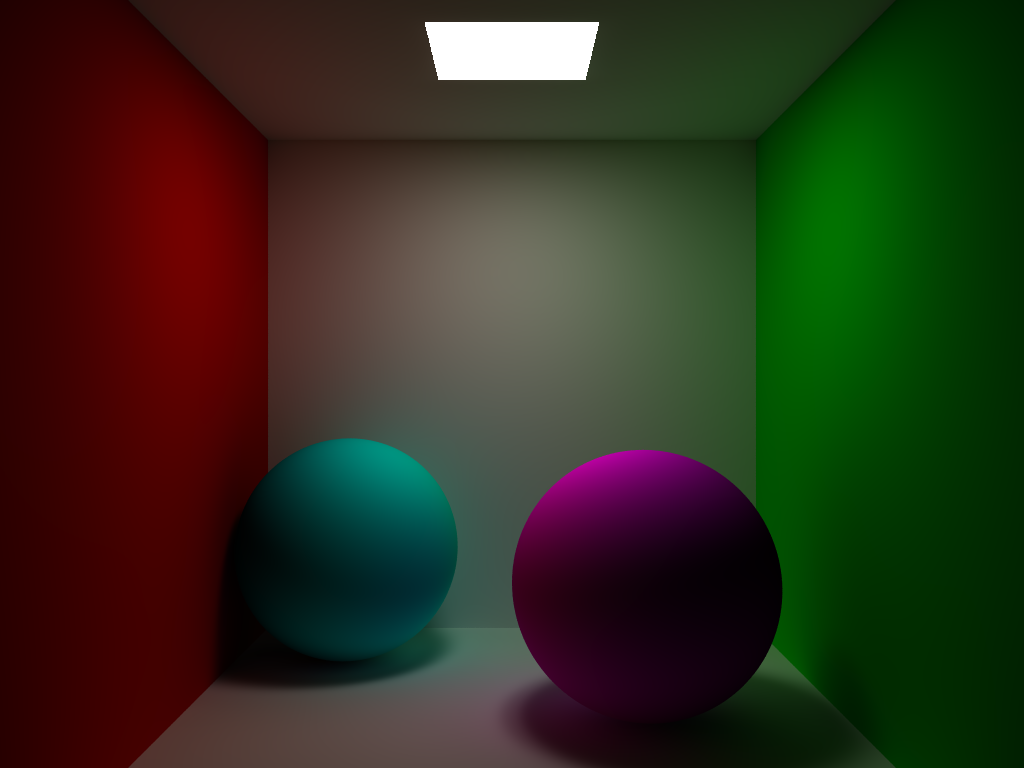
\includegraphics[width=\textwidth]{img/prediction.png}
        \caption{预测结果}
    \end{subfigure}
    \caption{Ground truth \& 预测结果}
    \label{fig:prediction_groundtruth}
\end{figure}